\documentclass[wcp]{jmlr}
% The following packages will be automatically loaded:
% amsmath, amssymb, natbib, graphicx, url, algorithm2e
%\usepackage{rotating}% for sideways figures and tables
\usepackage{longtable}% for long tables
\usepackage{subeqnarray}

\usepackage{cases}
\usepackage{booktabs}
\usepackage{graphics}
\usepackage{epstopdf}
\usepackage{amsmath,amssymb,amsfonts}
\usepackage{algorithm}
\usepackage{algorithmic}
\usepackage{verbatim}
\usepackage{makecell}
\usepackage{diagbox}
\usepackage{array}
\usepackage[justification=centering]{caption}
\usepackage{indentfirst}

% The following command is just for this sample document:
\newcommand{\cs}[1]{\texttt{\char`\\#1}}
\newcommand{\tabincell}[2]{\begin{tabular}{@{}#1@{}}#2\end{tabular}} 

\jmlrvolume{80}
\jmlryear{2018}
\jmlrworkshop{ACML 2018}

\title{ECG Classification with multi-scale features \\ based on unfixed-length Heartbeat-segmentation}
 % Use \Name{Author Name} to specify the name.
 % If the surname contains spaces, enclose the surname
 % in braces, e.g. \Name{John {Smith Jones}} similarly
 % if the name has a "von" part, e.g \Name{Jane {de Winter}}.
 % If the first letter in the forenames is a diacritic
 % enclose the diacritic in braces, e.g. \Name{{\'E}louise Smith}

 % Two authors with the same address
 % \author{\Name{Author Name1} \Email{abc@sample.com}\and
 %  \Name{Author Name2} \Email{xyz@sample.com}\\
 %  \addr Address}

 % Three or more authors with the same address:
  \author{\Name{Bin Chen} \Email{16120044@bjtu.edu.cn}\\
   \Name{Yuchun Guo} \Email{ychguo@bjtu.edu.cn}\\
   \Name{Yishuai Chen} \Email{yschen@bjtu.edu.cn}\\
   \addr Beijing Jiaotong University, Beijing, China}

 % Authors with different addresses:
%  \author{\Name{Author Name1} \Email{abc@sample.com}\\
%  \addr Address 1
%  \AND
%  \Name{Author Name2} \Email{xyz@sample.com}\\
%  \addr Address 2
% }

\editors{Jun Zhu and Ichiro Takeuchi}

\begin{document}

\maketitle
%***************************************************************%

\begin{abstract}
With the rapid spread of portable ECG monitoring devices, an accurate automatic arrhythmia classification system based on electrocardiogram (ECG) is of great significance. The existing studies focus on the choice of classifiers. They segment ECG beats by a given number of samples without considering that heartbeats are physiological patterns varying with temporal, personal, or contextual conditions and therefore are of unfixed-lengths. In this study, we first proposed a method to precisely segment an ECG beat with different number of samples based on its real length. Then, we shape it to a valid and fixed-length required by 1-D convolutional neural network (CNN). After that, we use 1-D CNN for the extraction of multi-scale features and classification. We validate our algorithm on the MIT-BIH dataset and follow AAMI recommendation for class labeling. Our method reach the accuracy of 96.25\%, the best of related work.
\end{abstract}
\begin{keywords}
ECG beats classification, multi-scale features, unfixed-length
\end{keywords}


\section{INTRODUCTION}
As the number of cardiovascular patients is increasing rapidly, the need for dynamic real-time monitoring of heart activity is also increasing. With the help of wearable or portable ECG monitoring devices, together with an automatic classification system, patients can be informed of ECG abnormalities in time. Though the existing automatic classification system of ECG beats has reached a high accuracy rate, there is still space to improve the classification accuracy.


An automatic classification system of ECG beats consists of three parts, the segmentation of ECG beats, the extraction of features and the classification of ECG beats. The segmentation of ECG beats means to parition each beat from a ECG continuous record. The extracted features are either hand-crafted manual ones or deep representation. The classic classifiers are SVM, random forest and neural network. \cite{raj2017ecg} use SVM,  \cite{li2016ecg} use random forest and \cite{hong2017encase} use 1-D CNN.


The existing work focuses on the extraction of features and the classification of ECG beats. They ignore the importance of the segmentation of ECG beats. Because the start and the end of an ECG beat are hard to determined, it is a routine to take R peak as a reference point and define an ECG beat to be a sequence of some samples before and after R peak. Each beat segmented in this way is of fixed-length, i.e. same number of samples. But heartbeats are physiological patterns varying with temporal, personal, or contextual conditions so that ECG beats are of different lengths. Segmenting ECG beats with fixed-length may result in the incompleteness of a heartbeat and even worse the redundancy of a heartbeat, i.e. the extra part of a previous or posterior beat.


Furthermore, \cite{xiang2018ecg} prove that the introduction of inner-beat features, i.e. the features of P wave, QRS waves and T wave, helps improve the classification accuracy. They obtain P wave, QRS waves and T wave by segmenting a single beat into three non-overlapping parts. However, the PQRST waves also vary with different conditions and are of unfixed-lengths so that the wave will draw the same loss as that for beat segmentation with fixed-length. The segmentation error will get worse as the basic segmentation is of fixed-length and not precise.


In addition to inner-beat and beat features, the inter-beat features that represent the correlation between ECG beats should be considered on classification. We define the inter-beat features as the related variations between ECG beats, such as the ratio of the beat lengths. By considering inter-beat features, the temporal dynamic relative changes of beats are utilized to help improve the classification performance.

  
To solve the above problems, we propose ECG classification with multi-scale features, including inner-beat, beat and inter-beat features. First, we redefine the length of an ECG beat and propose to segment ECG beats with unfixed-length. Second, based on our new algorithm of segmenting ECG beats, we introduce another algorithm to obtain the inner-beat waves precisely. Third, we use 1-D CNN to extract inner-beat and beat features. Then, we propose a new algorithm to extract inter-beat features and some traditional features. After that, we feed the inner-beat, beat and inter-beat features with traditional features into a fully connected neural network for classification. We evaluate our algorithm on the MIT-BIH dataset. We show the effect of the inner-beat, beat and inter-beat features on classification accuracy separately. Comparing with other related work, our method achieve a much better result.
  
  
The rest of this paper is organized as follows. In Section 2, we review the previous work. Our algorithm is explained in detail in Section 3. Section 4 presented experimental results. Finally, Section 5 concludes this paper.
\section{RELATED WORK}
As we mentioned before, The segmentation of ECG beats, the extraction of features and the classification of ECG beats make up an automatic classification system of ECG beats.


With the R peak as a reference point, all existing work, such as \cite{ye2012combining}, \cite{kiranyaz2016real}, \cite{zubair2016automated}, \cite{salloum2017ecg} and \cite{ye2012heartbeat}, extract ECG beats by a fixed-length. But the length of ECG beats varies because of different conditions or different individuals. it is clear that this segmentation is unreasonable. While, there are two reasons why this method is still widely used. On the one hand, it is hard to define the start and the end point of an ECG beat. On the other hand, the neural network requires a fixed input size. So all studies simplify the segmentation of ECG beats by a fixed-length. We are going to solve the problem in this paper by segment ECG beats with an unfixed-length and figure out how to shape ECG beats from an unfixed-length to a fixed-length.


Inner-beat features are proved to be useful on ECG beats classification. \cite{xiang2018ecg} introduce inner-beat features and prove that it is effective with experiments. They segment PQRST waves by dividing an ECG beat into three non-overlapping and fixed-length parts. But the length of wave also varies with time and person. Meanwhile, \cite{xiang2018ecg} use the above method to segment ECG beats, which is to obtain an ECG beat with a fixed-length. As such method may obtain an ECG beat even including the waves of the previous or posterior ECG beat, based on this, their method may get the P wave of the posterior beat when they actually want the T wave of the current beat. So it is necessary to find a better algorithm to obtain the waves.

Besides, though the concept of inter-beat feature was not been dicussed widely. There are only a few work taht consider this feature. \cite{xiang2018ecg} use RR intervals difference in their work. \cite{kiranyaz2016real} use the part of adjacent beats as another input of neural network. However, the inter-beat feature needs more investigation. So we are going to attempt to use other forms of inter-beat features.


As to the choice of classifiers, neural networks perform better than traditional classifiers such as SVM and random forest. \cite{jiang2007block} use a block-based neural network in 2007. \cite{abhinav2011clasification} use artificial neural network in their work. \cite{kiranyaz2016real} first propose to use 1-D convolutional neural network. \cite{zubair2016automated} and \cite{li2017classification} also use 1-D CNN. \cite{salloum2017ecg} use recurrent neural network. And \cite{limam2017atrial} use a deep neural network called convolutional recurrent neural network. Another thing worth noting is that, though all above work use neural network, the number of classifiers is different. \cite{kiranyaz2016real} train a classifier for each specific subject, while \cite{zubair2016automated} train a classifier for all subjects. Although a classifier for each specific subject can be of good accuracy for the same person,but not necessarily for another, especially a new patient. So we are going to training a classifier for all patients.
\section{METHOD}
In this section, We introduce our method that aims at extracting the multi-scale features of ECG beats, including inner-beat, beat and inter-beat features. The method includes four parts: the segmentation of ECG beats with unfixed-length (SEU), the overlapping segmentation of waves(OSW), the extraction of inter-beat features (EIF) and 1-D CNN.
\subsection{The Segmentation of ECG Beats with Unfixed-length}
In this part, we explain how to define the start and the end points of an ECG beat, how to define the heartbeat length, and how to shape the ECG beats with unfixed-length into that with fixed-length to 1-D CNN which requires fixed-length input.
\subsubsection{Disadvantages of Segmenting ECG beats with fixed-length}
To discuss the problem in detail, we firstly reproduce the algorithm that \cite{ye2012combining} used to show the current segmentation scheme. ECG beats are represented by 100 samples before R peak and 200 samples after R peak as shown in Fig.~\ref{Fig 1}. The ECG beats in subgraph (a) and (b) are extracted from one subject, and the ECG beat in subgraph (c) is extracted from another subject.It can be find that the length of ECG beats extracted from the same individual varies. It is obvious we compared the ECG beat in subgraph (a) with that in subgraph (b). The ECG beat in subgraph (b) contains the P wave of the posterior ECG beat. Meanwhile, the length of ECG beats extracted from different individuals varies even more if we compared the ECG beat in subgraph (a) with that in subgraph (c). The ECG beat in subgraph (c) even contains the R peak of the posterior ECG beat. So it is not reasonable to segment ECG beats with fixed number of samples.
\noindent
\begin{figure}[t]
\centering
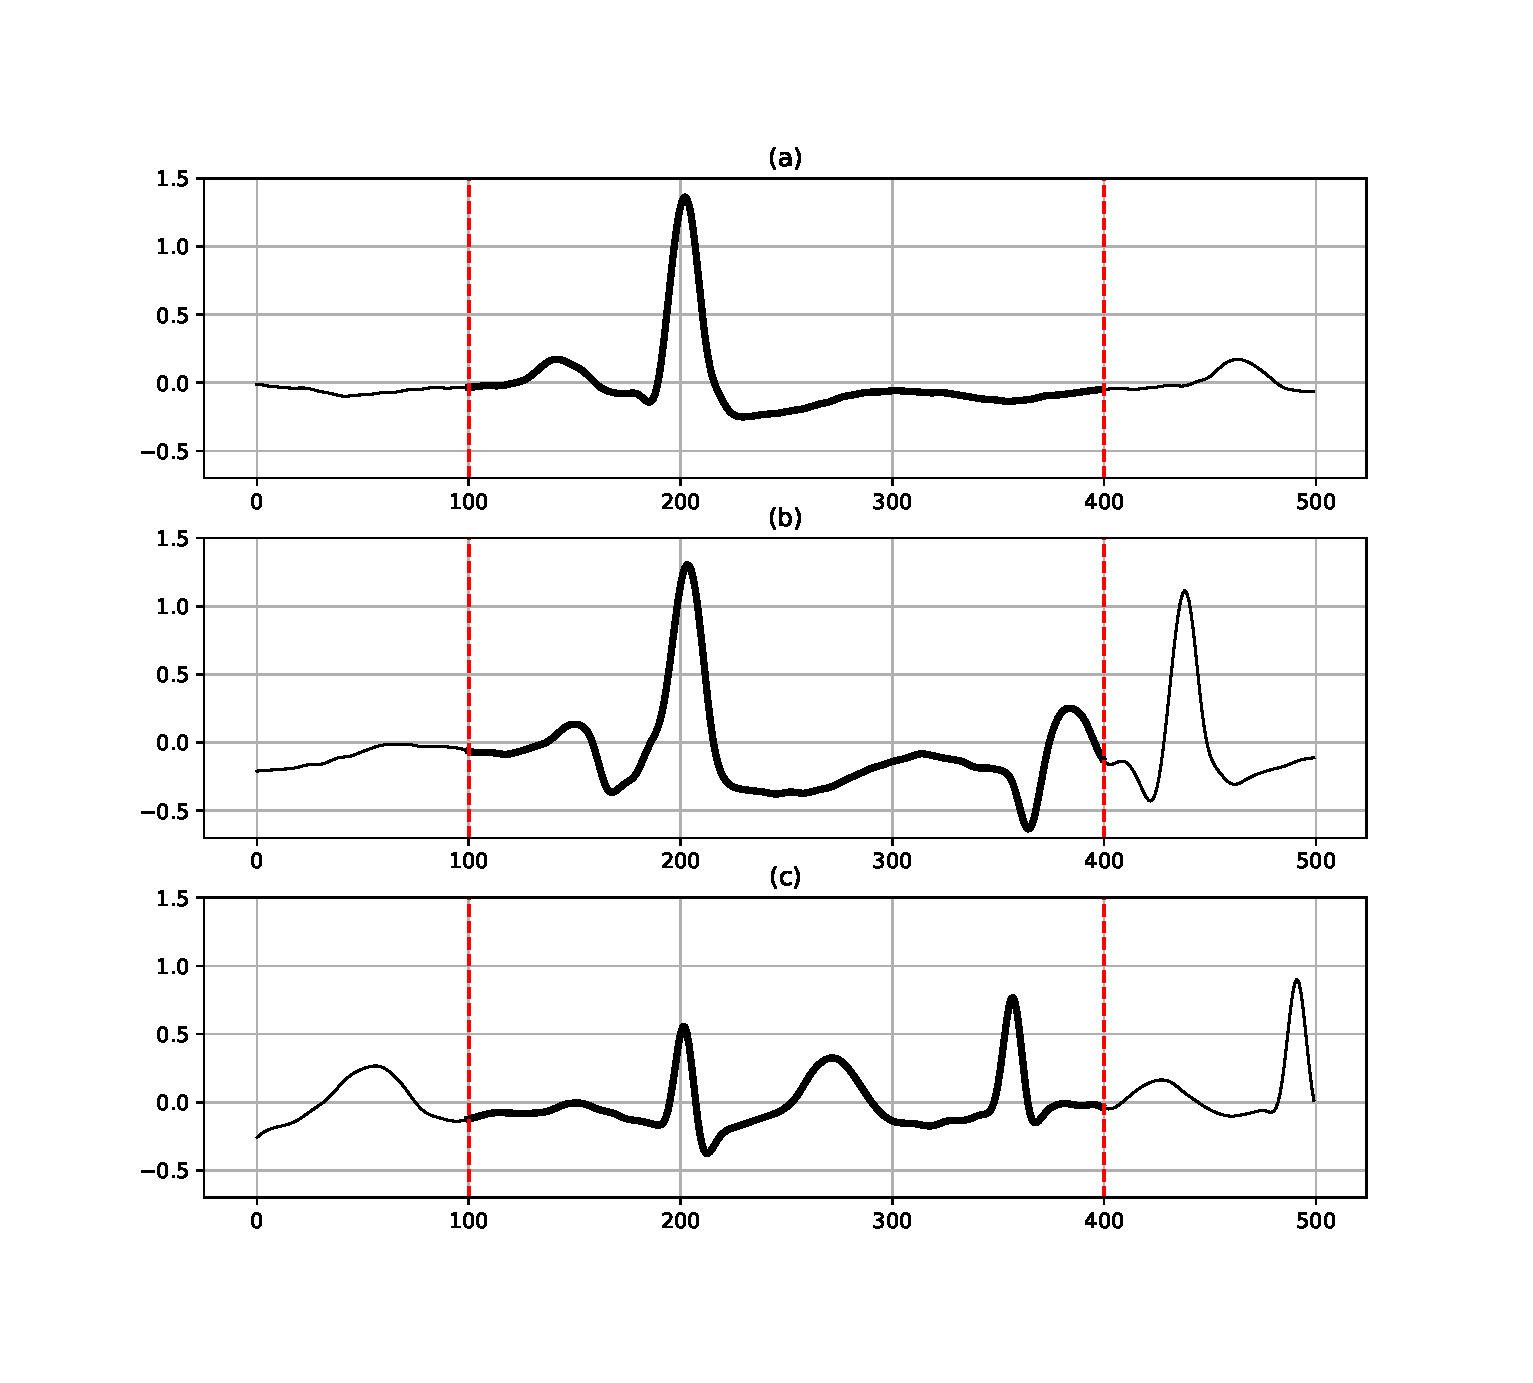
\includegraphics[scale=0.5]{frequency.eps}
\caption{The segmentation of ECG beats with fixed-length.}
\label{Fig 1}
\end{figure}
\subsubsection{Definition of the real length of ECG beat}
In order to express that the real length of ECG beats is changing, we need to redefine the real length of ECG beats. In Fig.~\ref{Fig 2}, three consecutive ECG beats is drawn for comparison of different segmentation scheme. 


As is shown, it is hard to determine the start and the end point of an ECG beat because boundaries of it is blurred with an algorithm or eyes of a human being without enough medical knowledge. But the R peak can be identified quickly and accurately by \cite{pan1985real}. Moreover, the length of the RR interval between the current R peak and the next R peak is also close to the real length of the current ECG beat. 


So we can define the real length of an ECG beat as the length of the RR interval, as shown by the black double-headed arrow in Fig.~\ref{Fig 2}. And the length of a RR interval is represented by a sequence of samples. Then, for the ECG beat $i$, we have
\begin{equation}
\label{Eq. 1}
  l_i = R_{i+1} - R_i
\end{equation}
where the $R_i$ means the index of the R peak of the ECG beat $i$ in a continuously time series, the $R_{i+1}$ means the index of R peak of the ECG beat $i+1$, and $l_i$ means the real length of the ECG beat $i$, i.e. the number of samples of ECG beat $i$. From Eq.~\ref{Eq. 1}, we obtain the real length of an ECG beat and it varies.
\subsubsection{Segment ECG beats with an offset}
While, it is unwise if we use the samples in a RR interval to represent an ECG beat directly. Because the samples between two R peaks is not a complete ECG beat. So how to get a real ECG beat?


Actually, we need to shift the start of the length leftward by $l_f$, then we obtain an real ECG beat like the red double-headed arrow in Fig.~\ref{Fig 2}. But what is the best value of $l_f$. We do a specific experiment and conclude that for MIT-BIH dataset. More details will be discussed in Section 4.
\noindent
\begin{figure}[t]
\centering
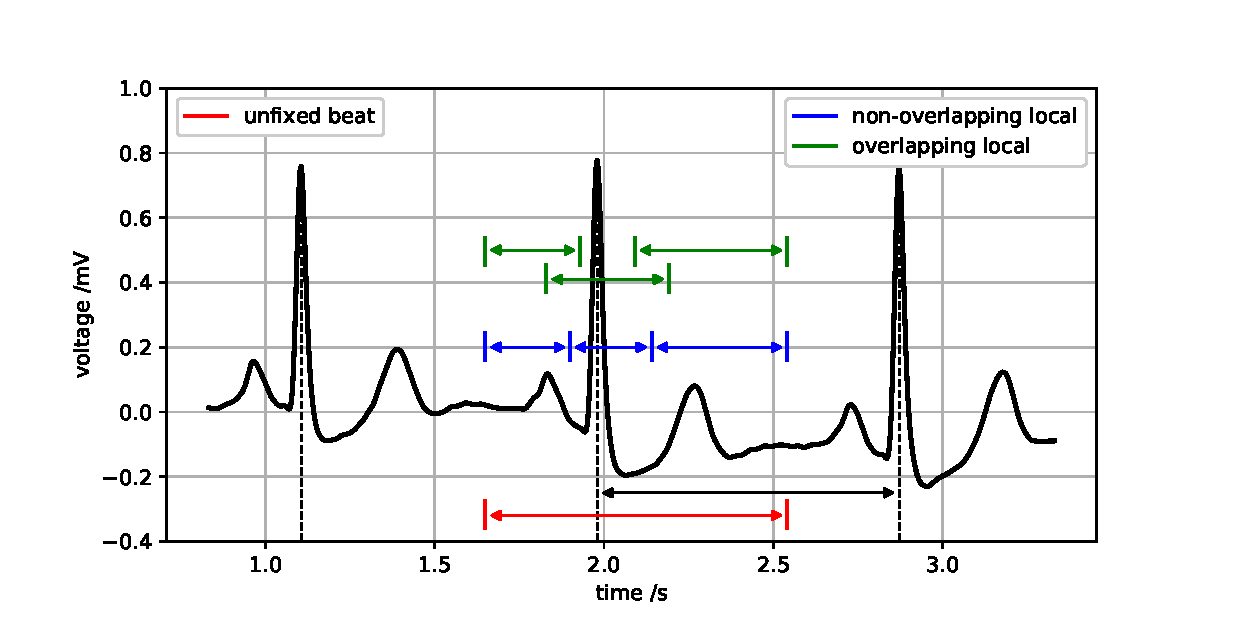
\includegraphics[scale=0.7]{beat.eps}
\caption{Segmentation of ECG beats.}
\label{Fig 2}
\end{figure}
\subsubsection{Shape ECG beats from unfixed-length to fixed-length}
Through the above two steps, we have obtained ECG beats, and the real length of each ECG beat is different. Whereas, this also brings us a new problem because the 1-D CNN needs input data of a fixed-length. So we need to shape our ECG beats of an unfixed-length to that of a fixed-length.


The most basic method is to set a parameter $L$ as the valid length. When the real length of an ECG beat is shorter than $L$, we add zeros at the tail of the ECG beat. Otherwise, we intercept the ECG beat at tail. Actually, there is no need to worry too much about the samples lost at the tail of the ECG beat. Because it has little useful information. The result of experiment will prove it and we discuss this in Section 4 in detail. 


Actually, $L$ is valid length of an ECG beat, and it is same for all ECG beats. But the choice of the $L$ should be careful and reasonable because we cannot have a complete ECG beat if $L$ is too small or we may obtain a complete ECG beat with too many zero at the tail. In Section 4, we will choose $L$ based on its distribution.\\


Above all, we obtain ECG beats with the fixed-length of $L$ as we follow the above three steps. Our algorithm SEU is describe in algorithm \ref{Alg 1}. In algorithm \ref{Alg 1}, $record$ is a continuous ECG signal, $peak$ is an array of the index of R peaks, $L$ is the valid length, $l_f$ is the offset length. From SEU, we obtain a set of ECG beats which have a fixed valid length, but an unfixed real length. That is the $l_i$ is different for different ECG beat, which is also called RR interval, but the $L$ is same for different ECG beats is same.
\subsection{The Overlapping Segmentation of Waves}
In this section, firstly, we discuss the Disadvantages of non-overlapping segmentation. Then we introduce our overlapping segmentation algorithm.
\subsubsection{Disadvantages of non-overlapping segmentation of waves}
\cite{xiang2018ecg} segment waves of an ECG beat as follow. First of all, they obtain an ECG beat with an fixed-length. Then, based on this, they divide an ECG beat into three non-overlapping part as shown in Fig.~\ref{Fig 2} by the three blue double-headed arrow lines. The three lines represent P wave, QRS waves and T wave. For example, if the length of an ECG beat is 300, P wave is represented by samples from 0 to 80, QRS waves are represented by samples from 80 to 160 and T wave is represented by samples from 160 to 300. 


As they segment ECG beats and waves in each beat with fixed-length, the disadvantages are obviously if we look back to Fig.~\ref{Fig 1}. Compared the ECG beat in subgraph (a) and the ECG beat in subgraph (c), no matter they set the parameter, they will regard the QRS wave of the posterior beat as T wave of current beat. Even worse, there are many samples like this in dataset, which means our neural network training on the wrong data.
\subsubsection{Segment waves with overlapping algorithm}
To obtain inner-beat features, we need to extract P wave, QRS wave and T wave respectively and precisely. However, similar to a single ECG beat, the boundaries of the waves are also not clear enough to detect automatically. 


Different from \cite{xiang2018ecg}, we propose an algorithm based on SEU that can increase the probability of extracting a complete wave by overlapping sampling. The core idea of our algorithm is to overlap sampling ECG beats. That means some samples represent two kind of waves with the three green double-headed arrow lines in Fig.~\ref{Fig 2}. For we already know the location of R peak, and we also know the distance between R peak and the start point, assuming it is 125 samples and the parameter $L$ is set to 300. QRS waves are represented by the samples from 75 to 175. P wave is represented by the samples from 0 to 100. And T wave is represented by the samples from 150 to 300. Then the length of P, QRS and T wave can be calculated by Eq.~\ref{Eq. 3}.

\begin{subequations}
\begin{numcases}{}
   L_P = n_P*L + L_o\\
   L_R = n_R*L + L_o\\
   L_T = n_T*L + L_o\\
   n_P + n_R + n_T + 2*\frac{L_o}{L}= 1
\end{numcases}
\label{Eq. 3}
\end{subequations}
where $L_P$, $L_R$, $L_T$ means the length of P wave, QRS waves and T wave. And $L_o$ is the overlapping length. $n_P$, $n_R$, $n_T$ are the parameters that represents the proportion of each wave in an ECG beat. And we can also obtain PQRST waves with fixed-length.\\


The OSW is described in algorithm \ref{Alg 2}. OSW returns P wave, QRS waves and T wave with a fixed-length. And the probability of extracting the waves completely and precisely is obviously much high than \cite{xiang2018ecg}.

\noindent
\begin{minipage}{.5\textwidth}
\centering
\begin{algorithm}[H]
\SetAlgoNoLine
\caption{SEU}
\label{Alg 1}
\KwIn{$record$, $peak$, $L$, $l_f$}
\KwOut{$DATA$}
%initialization\;
\For{$R_i$ in $peak$}{
    $l_i = R_{i+1} - R_i$\\
    offset $l_f$\\
    segment $ECG_i$ \\
    \eIf{$l_i <= L$  }{
        add zero at tail
    }{
        intercept at tail
    }
    $DATA$ append $ECG_i$
}
\end{algorithm}
\end{minipage}
\begin{minipage}{.5\textwidth}
\centering
\begin{algorithm}[H]
\SetAlgoNoLine
\caption{OSW}
\label{Alg 2}
\KwIn{$DATA$, $n_P$, $n_R$, $n_T$ $L$, $L_o$}
\KwOut{$P, QRS, T$}
compute $L_P, L_R, L_T$\\
\\
$L_P = n_P*L + L_o$\\
$L_R = n_R*L + L_o$\\
$L_T = n_T*L + L_o$\\
\\
\For{$ECG^i$ in $DATA$}{
    extract $QRS$ wave\\
    extract $P$ wave\\
    extract $T$ wave
}
\end{algorithm}
\end{minipage}

\subsection{The Extraction of Inter-beat Features}
We introduce how to extract inner-beat and beat features, and now we introduce an algorithm to obtain inter-beat features. RR interval is known as an effective feature to classify the ECG beats. Further, the ratio of two adjacent RR intervals can be used to express the correlation between ECG beats. In our algorithm, for ECG beat $i$, the ratio of two adjacent RR of intervals is defined as follows,
\begin{equation}\label{Eq. 5}
  r_i = \frac{l_{i-1}}{l_i} = \frac{R_i - R_{i-1}}{R_{i+1} - R_i}
\end{equation}
where $r_i$ represents the ratio of two adjacent RR intervals for ECG beat $i$, other parameters is same to before. 


\cite{xiang2018ecg} also use the the ratio of different RR intervals, but they use a nonlinear function. If we define our ratio as $r$, we define their ratio as $r_x$,then we have
\begin{equation}\label{Eq. 6}
  r_x = \frac{r - 1}{r + 1} = 1- \frac{2}{r+1}
\end{equation}


From the Eq.~\ref{Eq. 6}, it is clear that $r_x$ is in fact a nonlinear function of $r$. In Fig.~\ref{Fig 3}, we set $r$ from 0.5 to 1.5 because most values of $r_i$ are in this interval. It is clear that the curve is a nonlinear function of $r$. 


Meanwhile, the real length of the current ECG beat, which is $l_i$, also named RR interval, is a manual feature to be used in the network.
\subsection{1-D CNN}
Convolutional neural networks have excellent performance in various tasks of images processing, such as image classification and object recognition. A classic convolutional neural work has two function, including feature extraction and classification. And the one-dimensional convolutional neural network is mainly to process sequence signals including time series. Obviously, 1-D CNN is very suitable to solve our ECG beats classification problem. It help us to learn some deep representation of ECG beats.
\section{EXPERIMENTS}
In this section, extensive experiments will be done to evaluate the algorithms we proposed. To show the effects of beat features extracted via SEU, we run two groups of experiments. The first one is to find the best offset described in section 3.1. The second one is to compare segmenting ECG beats with fixed-length and SEU. And to show the effects of inner-beat features extracted via OSW, is to compare SEU and SEU combined with OSW. Then to show the effects of inter-beat features extracted via EIF, we run experiments to compare the network with or without EIF. In order to avoid the random effect on the results, we preformed all experiments 10 times, and then calculated the mean.
\subsection{Dataset}
The ECG dataset from MIT-BIH arrhythmia database is used, which is considered as one of most famous standard database. The dataset contains 48 half-hour excerpts of two-channel ambulatory ECG recordings, obtained from 47 subjects studied by the BIH Arrhythmia Laboratory between 1975 and 1979. All recordings are passed through a band pass filter at 0.1-100Hz and are sampled at 360Hz. According to AAMI recommended practice, 4 paced beats, including 102, 104, 107 and 217, are excluded in this study because these beats do not preserve sufficient signal quality for reliable processing. So, 44 records from MIT-BIH arrhythmia database are selected to use for training and evaluating the proposed method. AAMI recommendation for class labeling is also adopted in this study. AAMI recommends that each ECG beat is classified into the following five beat types: N (normal beats), S (supraventricular ectopic beats), V (ventricular ectopic beats), and F (fusion beats), and Q (unclassifiable beats). For all records, modified-lead \uppercase\expandafter{\romannumeral2} signals are used.


To achieve ECG beats classification, we use 44 records from MIT-BIH arrhythmia database as we mentioned above. First of all, we need to filter all records, mainly including low-pass, trap filtering and zero-phase filtering. These three filters are used to eliminate the dataset of myoelectric interference, power frequency interference and baseline drift. Since the IIR filter is used, it produces a delay phenomenon, we need to do a left shift on the filtered data. The offset number is set to 72 samples based on experience.


There are more than 100 thousand beats we need to classify to five types recommended by AAMI. Similar to \cite{zubair2016automated}, from the first 20 record (100-124) of the MIT-BIH database, 75 beats are randomly selected from each type-N, type-S and type-V beats and all beats of type-F and type-Q are selected. A set of these 245 beats and the beats from the first 5 minutes of the second 24 record (200-232) are used for training. Actually, no more than 10\% beats of the dataset are used for training. All the other beats are used as test dataset. And we randomly select five thousand from the test dataset as validation dataset. In all experiments, we adopt the same dataset partitioning method described above. Because the sampling frequency of all records is same, in the following parts, we still use the number of samples to represent time.
\noindent
\begin{figure}
\begin{center}
\begin{minipage}[c]{0.5\textwidth}
\centering
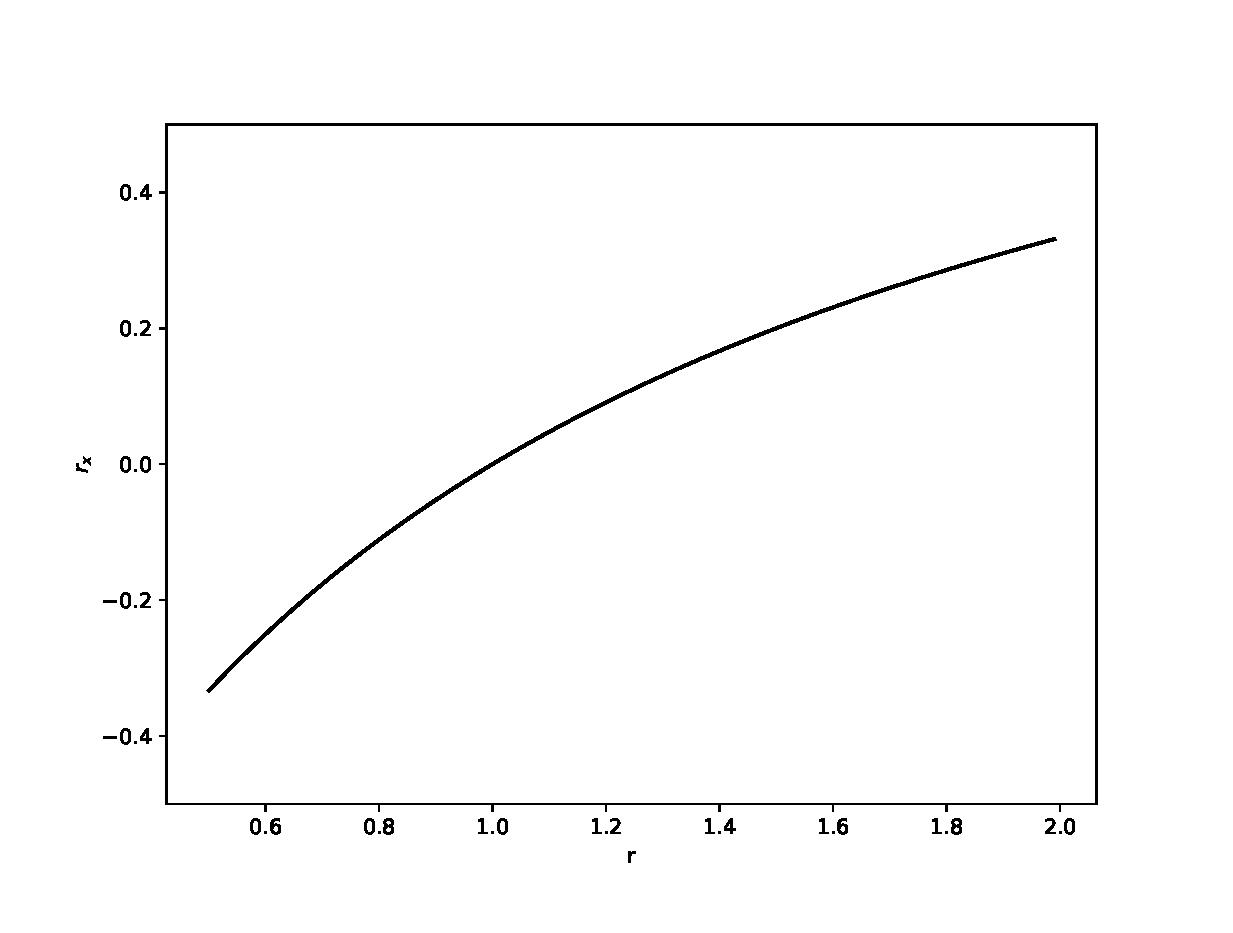
\includegraphics[angle=0,width=7cm,height=5cm]{gamma.eps}
\centering
\caption{The comparison of \\two kinds of ratio.}
\label{Fig 3}
\end{minipage}%
\begin{minipage}[c]{0.5\textwidth} 
\centering
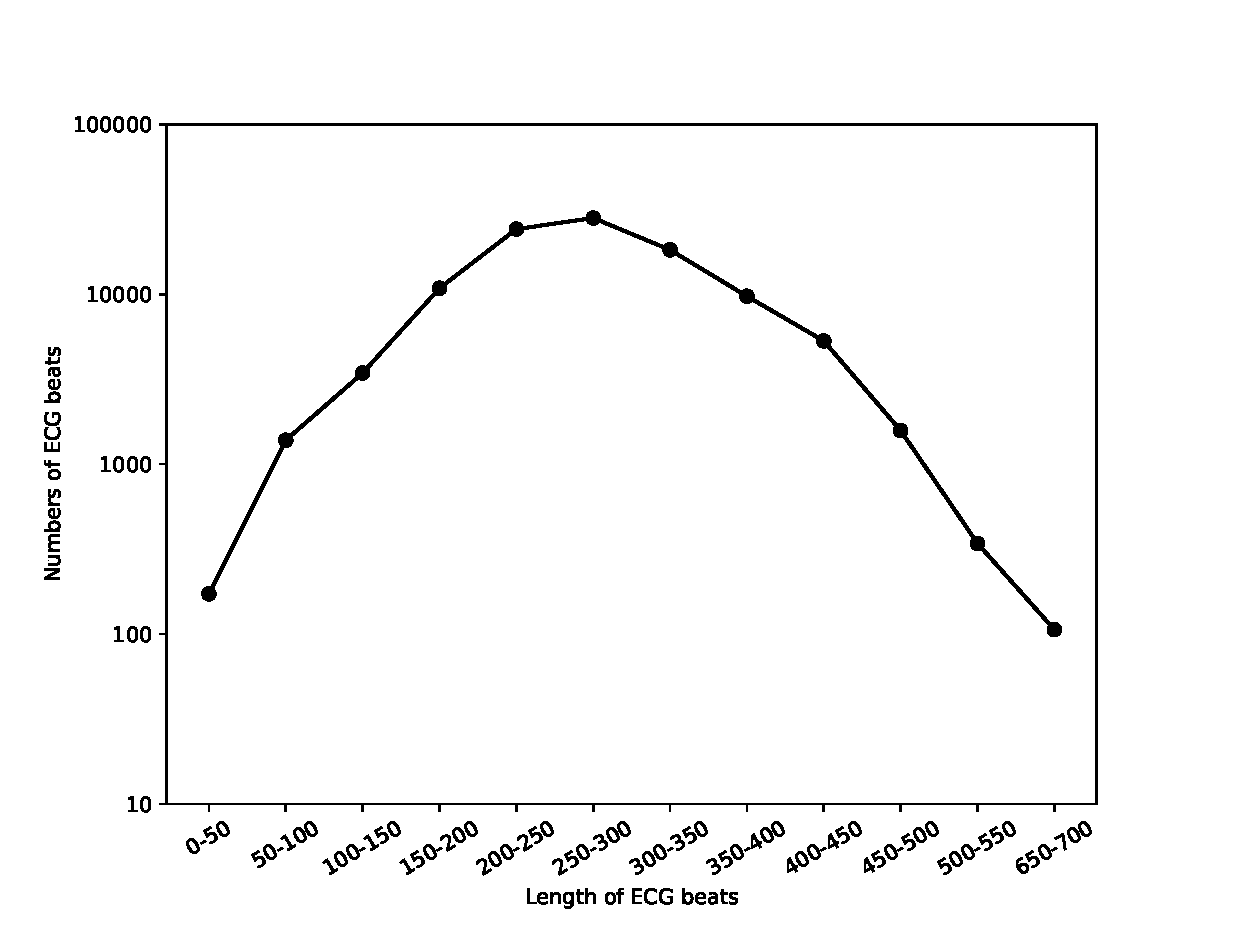
\includegraphics[angle=0,width=7cm,height=5cm]{distribution_line.eps}
\caption{Distribution of the length \\of ECG beats.}
\label{Fig 6}
\end{minipage}
\end{center}
\end{figure}
\subsection{Effects of Beat Features Extracted via SEU}
\subsubsection{Setup}
In this experiment, we use a simple 1-D CNN consists of three convolutional units and a MLP layers and a softmax layer. The convolutional unit is shown in subgraph (a) of Fig.~\ref{Fig 4}. A convolutional unit consists of a convolutional layer (conv), a dropout layer, a maxpooling layer (MP) and a batch normalization layer (BN). The structure of the 1-D CNN is shown in subgraph (b) of Fig.~\ref{Fig 4}. The cells of different convolutional units and MLP layer are indicated in parentheses. The parameter of dropout layer is set to 0.2. The pooling size is set to 2. What have to be aware of is that in the CONV\_1, we do not use a dropout layer. And to avoid overfitting, we also add a dropout layer after the MLP layer. And we also use L2 regularization at softmax layer to avoid overfitting.
\noindent
\begin{figure}
\begin{center}
\begin{minipage}[c]{0.5\textwidth}
\centering
\includegraphics[angle=0,width=7cm,height=6cm]{1.eps}
\centering
\caption{1-D CNN for beat features\\ extraction.}
\label{Fig 4}
\end{minipage}%
\begin{minipage}[c]{0.5\textwidth} 
\centering
\includegraphics[angle=0,width=7cm,height=6cm]{2.eps}
\caption{1-D CNN for inner-beat and \\beat features extraction.}
\label{Fig 5}
\end{minipage}
\end{center}
\end{figure}
\subsubsection{Choice of Offset}
In this experiment, we will set the offset to different values and test the performance on the test set. The value of the offset is set to 25, 50, 75, 100, 125, and 150 in sequence. Another parameter that needs to note is the value of $L$. We choose the parameter by analysing the actual situation of the database. Fig.~\ref{Fig 6} shows that the distribution of the length of ECG beats in the MIT-BIH dataset. In Fig.~\ref{Fig 6}, 50 is used as an interval, and all ECG beats fall into the corresponding interval based on their length, after that we count the number of ECG beats of each interval. The line indicates the number of ECG beats in each interval. Actually, the intervals whose the number of ECG beats is less than 100 are not shown in Fig.~\ref{Fig 6}. In this experiment, we choose the top one interval to represent $L$. As we used batch normalization in our network, so we set the number of epochs to 15.


The results of the experiment are shown in Fig.~\ref{Fig 7}. We plot ten times result of each value of offset, and the black line represents the mean of ten times. Fig.~\ref{Fig 7} shows intuitively that when we set the $L$ to 300, the offset of 125 has the best test results.
\noindent
\begin{figure}
\centering
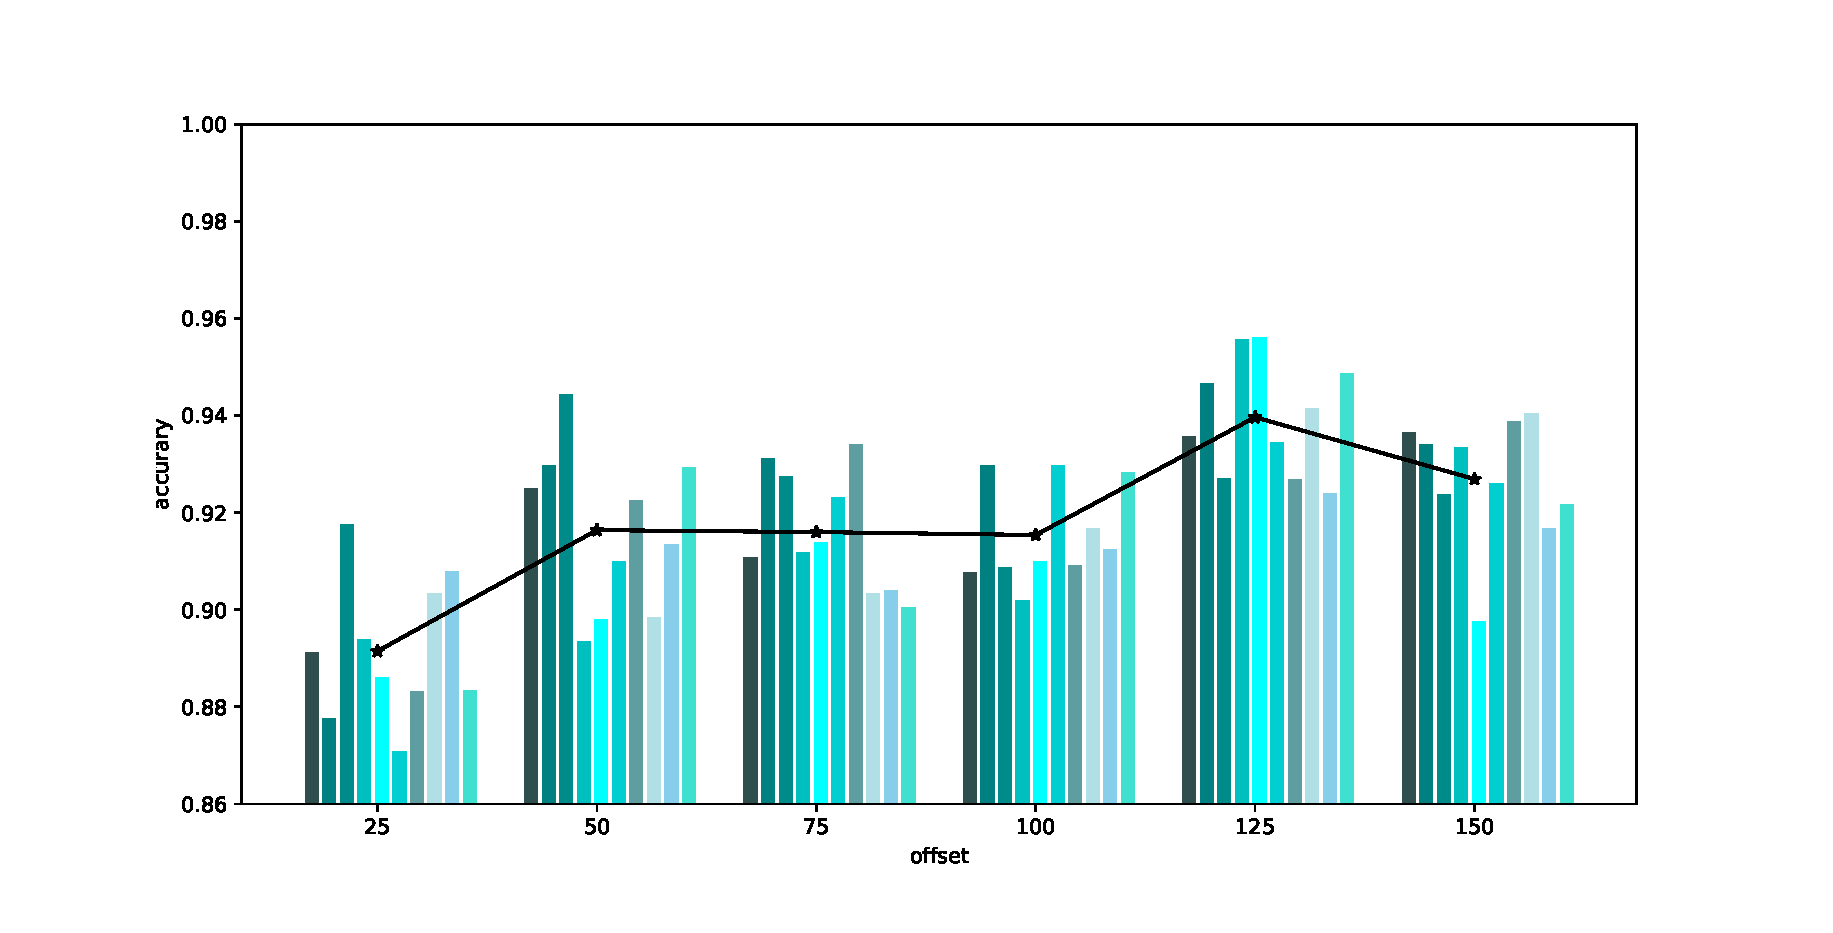
\includegraphics[scale=0.5]{offset.eps}
\caption{The accuracy of  results of offset.}
\label{Fig 7}
\centering
\end{figure}
\subsubsection{Effects of the Valid Length}
In this experiment, we evaluate SEU and the segmentation algorithm with fixed-length. To prove the results of SEU are stable and effective, we choose the top 3 of the numbers of $L$ to represent the length of an ECG beat, which are 250, 300, and 350. And for comparing to the segmentation algorithm with fixed-length, we also set $L$ with the same numbers. And the offset is correspondingly set to 100, 125 or 150. So, 150, 175 or 200 samples are extracted after R peak. Same to the above experiment, the epoch is also set to 15.


Our results are showing in Tab.~\ref{Tab 1}.It is obvious that our algorithm is superior to the segmentation algorithm with fixed-length on every value of $L$, especially when $L$ is 300. Meanwhile, SEU is more stable than the segmentation algorithm with fixed-length. The maximum difference of SEU is 0.00539, while the other one is 0.009, about 1.7 times than SEU.


There is also an interesting phenomenon that SEU performs best when $L$ is 300. As we mentioned in Section 3, although we can obtain more complete ECG beats if we increase the parameter $L$, for those ECG beats whose length is shorter than parameter $L$, the zeros at their ending also increase, which increases the invalid samples of the ECG beats. When $L$ is greater than 300, the income of the former is less than the loss of the latter. So this is why we cannot set $L$ as big as we can.
\\

\noindent
\begin{minipage}{\textwidth}
 \begin{minipage}[t]{0.5\textwidth}
  \centering
   %\raggedleft
     \makeatletter\def\@captype{table}\makeatother\caption{The experimental result of different L.}
     \label{Tab 1}
       \begin{tabular}{|c|c|c|c|} 
		\hline 
		$L$&250&300&350\\
		\hline  
		fixed&0.93091&0.92191&0.92965\\
		\hline 
		USEBS&{\bf 0.93474}&{\bf 0.93965}&{\bf 0.93426}\\
		\hline
	\end{tabular}
  \end{minipage}
  \begin{minipage}[t]{0.5\textwidth}
   \centering
    %\raggedright
        \makeatletter\def\@captype{table}\makeatother\caption{The experimental result of inner-beat features.}  
        \label{Tab 2} 
         \begin{tabular}{|c|c|c|c|}
         \specialrule{0em}{0pt}{0pt}
          \hline 
		algorithm&SEU&\tabincell{c}{SEU\\+OSW}&\tabincell{c}{fixed\\+OSW}\\
		\hline  
		accuracy&0.93965&{\bf 0.94816}&0.92498\\
		\hline
	  \end{tabular}
   \end{minipage}
\end{minipage}

\subsection{Effects of Inner-beat Features Extracted via OSW}
\subsubsection{Setup}
The convolutional neural network without inner-beat features is same to the experiment effect of SEU, and convolutional neural network with inner-beat features is a multiple input single output network as shown in Fig.~\ref{Fig 5}. To learn inner-beat features, we use two convolutional units, and to learn beat features, we use three convolutional units. Then we concatenate the features learned by the different part of convolutional neural network and feed it into a network with two MLP layers and a softmax layer. To avoid overfitting and speed up training process, not only dropout but also batch normalization and regularization are used in our network. All important parameters are indicated in parentheses. Similar to before, the first convolutional unit does not have a dropout layer. A batch normalization layer is add after each MLP layer.
\subsubsection{Experimental Results}
As we mentioned before, it is hard to extracted PQRST waves precisely, so we solve the problem by using OSW. The value of the parameter $L$ is set to 300. $n_P$ is set to 0.25. $n_R$ is set to $\frac{1}{6}$. $n_T$ is set to $\frac{5}{12}$. And $L_o$ is set to 25. The mean of accuracy of ten times of the experiment is shown in Tab.~\ref{Tab 2}. We also comparing the result with the method which extracts inner-beat and beat features by fixed-length. It is obvious that the results of SEU and OSW is much better than others. We also show the results of the ten times experiments in Fig.~\ref{Fig 8}. From the Fig.~\ref{Fig 8}, it is obviously SEU+OSW is better than other algorithms except three times i.e. 5, 6 and 8 because the CNN has a little randomness. 
\noindent
\begin{figure}
\centering
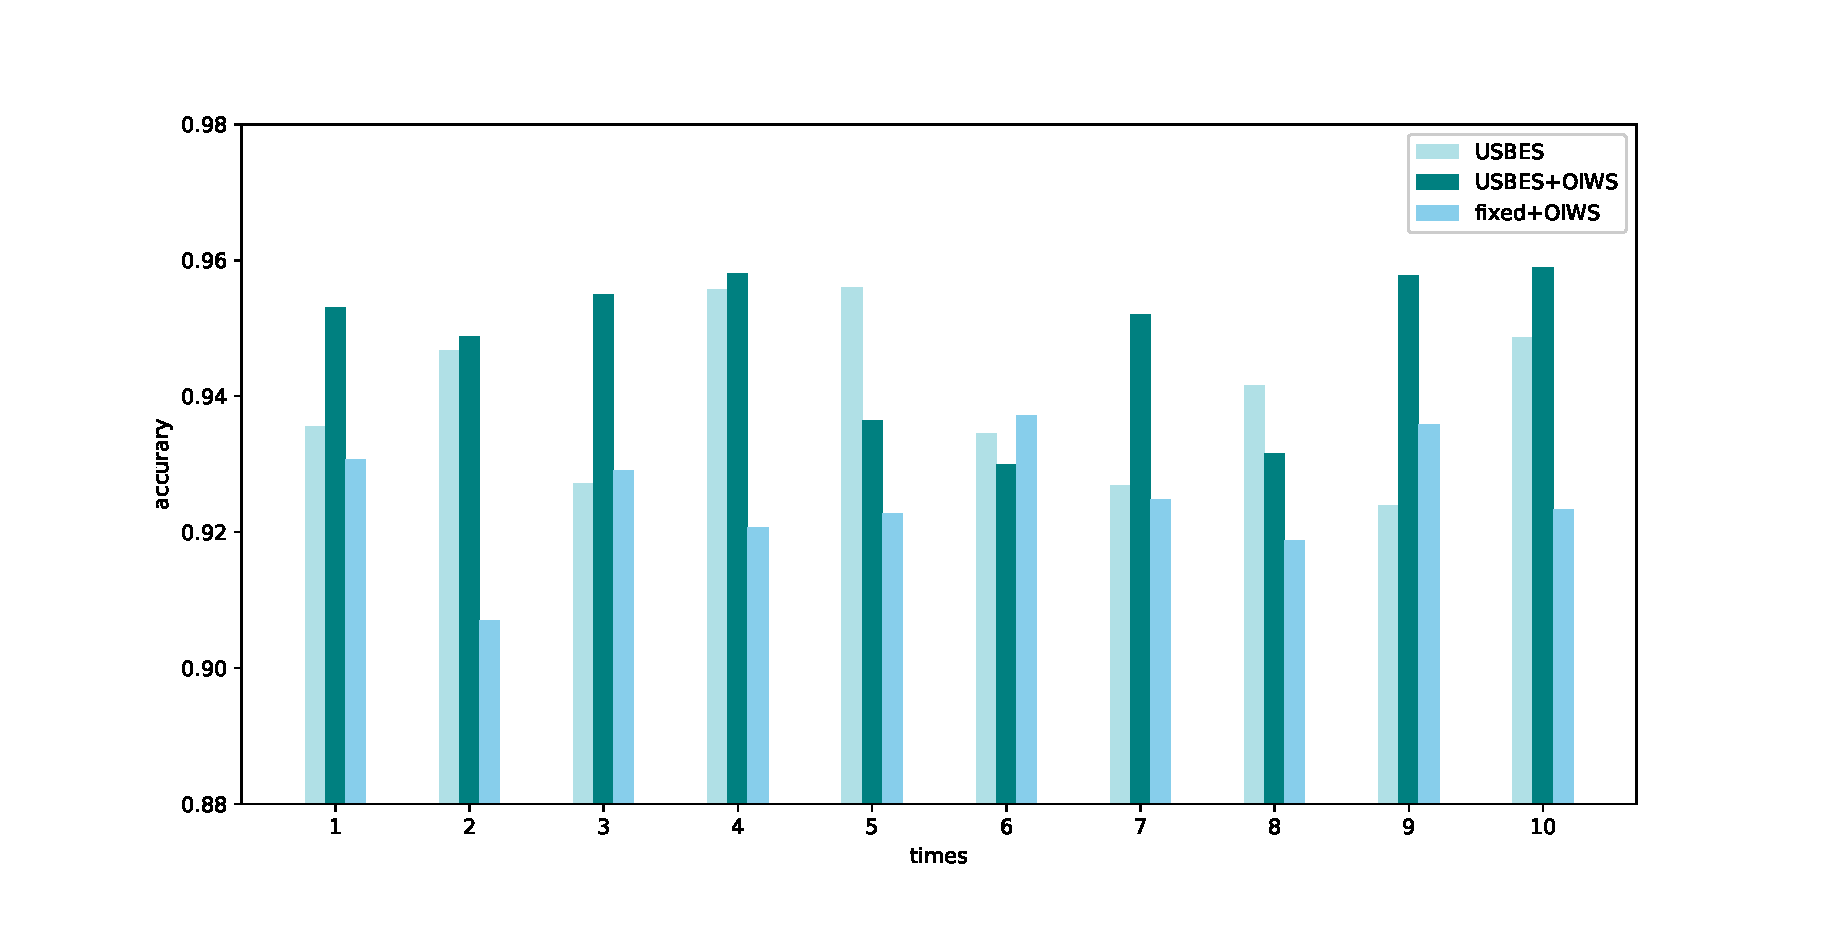
\includegraphics[scale=0.5]{inner-beat.eps}
\caption{The ten times experimental results of inner-beat features.}
\label{Fig 8}
\centering
\end{figure}
\subsection{Effects of Inter-beat Features Extracted via EIF}
\subsubsection{Setup}
The network of this experiment is similar to Fig.~\ref{Fig 5}. What is different is that we add an inter-beat feature and a manual feature at concatenate layer.
\subsubsection{Experimental Results}
As we mentioned before, two features, the ratio two adjacent RR intervals and the length of current RR interval, are fed into concatenate layer. The mean of ten times of the experiment is shown in Tab.~\ref{Tab 3}.


It is obvious that the inter-beat feature and the manual feature are effective to improve accuracy in Tab.~\ref{Tab 3}. The best accuracy of 10 times of the experiment is 0.9625, and the confusion matrix of ECG beats classification for test data is shown in Tab.~\ref{Tab 4}. On the one hand, in order to make model more generalizable, regularization is used. On the other hand, there are more than 10000 samples but only 7 samples of Q type in training set. This explains why the last column of the confusion matrix is all 0. Fortunately, Q type, which is unclassifiable beats, is less important than the other four types, so there is no need to worry about this. The comparison of our work with other existing methods is given in Tab.~\ref{Tab 5}. It can be see that our study has a significant improvement on the accuracy of classification.
\noindent
\begin{table}[H]
\centering
\caption{The experimental result of inter-beat features.}
\begin{tabular}{|c|c|c|} %l(left)居左显示 r(right)居右显示 c居中显示
\specialrule{0em}{0pt}{0pt}
\hline 
EIF&with&without\\
\hline  
accuracy&{\bf 0.95451}&0.94816\\
\hline 
\end{tabular}
\label{Tab 3}
\end{table}
\noindent
\begin{minipage}{\textwidth}
 \begin{minipage}[t]{0.5\textwidth}
  \centering
   %\raggedleft
     \makeatletter\def\@captype{table}\makeatother\caption{Confusion matrix.}
     \label{Tab 4}
       \begin{tabular}{|c|c|c|c|c|c|}
		\hline
		\diagbox{T}{P}&N&S&V&F&Q\\ %添加斜线表头
		\hline
		N&75728&109&780&21&0\\
		\hline
		S&1048&1200&147&0&0\\
		\hline
		V&623&181&4899&43&0\\
		\hline
		F&189&1&40&257&0\\
		\hline
		Q&7&1&4&2&0\\
		\hline
		\end{tabular}
  \end{minipage}
  \begin{minipage}[t]{0.5\textwidth}
   \centering
    %\raggedright
        \makeatletter\def\@captype{table}\makeatother\caption{The comparison of related work.}
        \label{Tab 5}
         \begin{tabular}{ccc}
		%\diagbox{T}{P}&N&S&V&F&Q\\ %添加斜线表头
		\specialrule{0em}{0pt}{2pt}
		\hline
		Methods&Year&Acc\\
		\hline
		\cite{jiang2007block}&2013&85\%\\
		\hline
		\cite{li2017classification}&2014&91.7\%\\
		\hline
		\cite{zubair2016automated}&2016&92.7\%\\
		\hline
		\cite{ebrahimzadeh2016classification}&2017&93.08\%\\
		\hline
		\cite{acharya2017deep}&2017&93.47\%\\
		\hline
		Proposed&-&{\bf 96.25}\%\\
		\hline
		\end{tabular}
   \end{minipage}
\end{minipage}
\section{CONCLUSION}
In this paper, we have proposed an automatic classification system of ECG beats and verified its performance with extensive experiments. The results show that: 1) the SEU algorithm, based on the real and the valid ECG beats length, dramaticlly improved the accuracy about 1.8\% than fixed-length, when the valid length is 300 samples; 2) together with the SEU, OSW algorithm improved the accuracy about 0.9\%, up to 94.82\%; 3) the introduction of EIF algorithm in our system further improved about 0.6\%; 4) the best accuracy of our method is up to 96.25\%, which is about 3\% higher than existing related work.



For the feature work, we will investigate three issues. First of all, other representation of offset and waves can be considered. Then, many other inter-beat features can be examined. Finally, recurrent neural network and convolutional recurrent neural network can also be considered as neural network classifiers.
\acks{}
This work was supported in part by the National Science Foundation of China under Grant No. 61572071,61271199, 61301082.
\bibliography{acml18}
\end{document}